\documentclass[10pt,journal]{IEEEtran}
\usepackage[utf8]{inputenc}
\usepackage[T1]{fontenc}
\usepackage{lmodern}
\usepackage{microtype}
\usepackage{amsmath,amssymb,amsthm,mathtools,bm}
\usepackage{algorithm}
\usepackage{algpseudocode}
\usepackage{booktabs,longtable,tabularx,multirow,array}
\usepackage{graphicx,subcaption,float}
\usepackage{tikz}
\usepackage{enumitem}
\usepackage{xcolor}
\usepackage{hyperref}
\usepackage[capitalise,noabbrev]{cleveref}
\usepackage[numbers,sort&compress]{natbib}
\usepackage{xparse}
\usepackage{balance}
\usetikzlibrary{arrows.meta,calc,positioning,shapes.geometric}
\graphicspath{{generated/}{../assets/figures/}{../../paper/assets/figures/}{../../reports/publication/}{../../reports/hil/}{../../reports/figures/}{../../reports/universal_orius_validation/}{../../reports/universal_training_audit/}}

\theoremstyle{plain}
\newtheorem{theorem}{Theorem}[section]
\newtheorem{proposition}[theorem]{Proposition}
\newtheorem{lemma}[theorem]{Lemma}
\newtheorem{corollary}[theorem]{Corollary}
\theoremstyle{definition}
\newtheorem{definition}[theorem]{Definition}
\newtheorem{assumption}{Assumption}
\theoremstyle{remark}
\newtheorem{remark}[theorem]{Remark}

\newcommand{\zt}{z_t}
\newcommand{\ztt}{\tilde{z}_t}
\newcommand{\ot}{o_t}
\newcommand{\xt}{x_t}
\newcommand{\wt}{w_t}
\newcommand{\dt}{d_t}
\newcommand{\st}{s_t}
\newcommand{\Chat}{\hat{C}_t}
\newcommand{\Crac}{\hat{C}_t^{\mathrm{RAC}}}
\newcommand{\Ut}{U_t}
\newcommand{\astar}{a_t^{*}}
\newcommand{\asafe}{a_t^{\mathrm{safe}}}
\newcommand{\Aset}{\mathcal{A}_t}
\newcommand{\dcs}{DC3S}
\newcommand{\oqe}{OQE}
\newcommand{\rac}{RAC-Cert}
\newcommand{\SOC}{\mathrm{SOC}}
\newcommand{\Emax}{E_{\max}}
\newcommand{\Pmax}{P_{\max}}
\newcommand{\Rmax}{R_{\max}}
\newcommand{\TSVR}{\mathrm{TSVR}}
\newcommand{\IR}{\mathrm{IR}}
\newcommand{\OASG}{\mathrm{OASG}}
\DeclareMathOperator*{\argmin}{arg\,min}
\DeclareMathOperator*{\argmax}{arg\,max}
\DeclareMathOperator{\Prob}{\mathbb{P}}
\newcommand{\E}{\mathbb{E}}
\newcommand{\R}{\mathbb{R}}

\newcommand{\ORIUSReuseInput}[1]{%
  \begingroup
  \let\ORIUSOriginalSection\section
  \let\ORIUSOriginalSubsection\subsection
  \let\ORIUSOriginalSubsubsection\subsubsection
  \ProvideDocumentCommand{\chapter}{s m}{%
    \IfBooleanTF{##1}{\ORIUSOriginalSection*{##2}}{\ORIUSOriginalSection{##2}}%
  }%
  \RenewDocumentCommand{\section}{s m}{%
    \IfBooleanTF{##1}{\ORIUSOriginalSubsection*{##2}}{\ORIUSOriginalSubsection{##2}}%
  }%
  \RenewDocumentCommand{\subsection}{s m}{%
    \IfBooleanTF{##1}{\ORIUSOriginalSubsubsection*{##2}}{\ORIUSOriginalSubsubsection{##2}}%
  }%
  \setlength{\textwidth}{\columnwidth}%
  \setlength{\linewidth}{\columnwidth}%
  \input{#1}%
  \endgroup
}


\title{ORIUS: A Professor Review Draft on Universal Runtime Safety for Physical AI under Degraded Observation}
\author{Author details omitted for professor review draft}
\date{}

\begin{document}
\maketitle

\begin{abstract}
ORIUS treats degraded observation as the fundamental hidden hazard for Physical AI:
controllers act on telemetry, beliefs, and summaries of the world, while safety is
judged on the physically true state. This manuscript presents ORIUS, Observation--
Reality Integrity for Universal Safety, as a reusable runtime layer that detects
reliability collapse, inflates the observation-consistent state set, tightens the
admissible action set, repairs or replaces unsafe actions, and emits auditable
certificates before release. The paper is organized around the universal runtime
claim rather than a witness-row-specific forecasting claim.
Its scientific object is a shared runtime grammar grounded in one adapter contract, one
benchmark schema, one CertOS governance surface, and one theorem bridge. Battery
remains the witness row with the deepest theorem-to-code-to-artifact closure; AV,
industrial, and healthcare are defended bounded rows; navigation and aerospace remain
explicitly gated by missing real-data closure. The central claim is therefore strong
but disciplined: ORIUS establishes a universal runtime safety layer for Physical AI
under degraded observation, while equal-domain empirical closure remains a governed
target rather than a present-tense fact.
\end{abstract}

\begin{IEEEkeywords}
Physical AI safety, degraded observation, observation--action safety gap, runtime
assurance, conformal uncertainty, safety filters, cyber-physical systems, certificates
\end{IEEEkeywords}

\section{Introduction and Contribution Statement}
\label{sec:prof-introduction}

Physical AI systems do not act on truth. They act on telemetry, inferred state, delayed
measurements, missing packets, stale buffers, and learned surrogates of the world. The
resulting engineering problem is deeper than forecast error or planner suboptimality:
the software stack can remain internally coherent while the physical system becomes
externally unsafe. Batteries may violate hidden state-of-charge limits, vehicles may
enter unsafe headway regimes on stale perception, industrial plants may cross thermal
or pressure envelopes, clinical monitoring pipelines may suppress timely intervention,
and navigation or flight systems may remain locally consistent while drifting outside a
feasible corridor.

ORIUS is built around the claim that these failures share one universal object:
degraded observation changes the semantics of what may still be safely done. The field
therefore needs a runtime layer whose job is not to outperform every planner, but to
mediate the boundary between degraded observation and physical actuation. ORIUS,
Observation--Reality Integrity for Universal Safety, is proposed as that layer. It
detects reliability loss, calibrates the observation-consistent state set, constrains
the admissible action set, repairs or replaces unsafe candidate actions, and certifies
release through an auditable lifecycle. The framework is written around the universal
runtime claim rather than a witness-row-specific framing. Battery is retained as the
deepest witness row, not as the conceptual center of the claim.

This manuscript positions ORIUS against a precise gap in the literature. Distribution-
free inference can quantify uncertainty
\cite{vovk2005algorithmic,lei2018distribution,romano2019conformalized,gibbs2021adaptive,angelopoulos2023gentle,barber2023beyond}.
Runtime assurance and shields can intercept unsafe behavior
\cite{sha1998simplex,sha2001using,desai2019soter,bloem2015shield,bartocci2018introduction,leucker2009brief}.
Safety filters and constrained control can map uncertainty into admissible action sets
\cite{ames2019control,ames2014cbf,wabersich2021predictive,fisac2019general,mayne2005robust,rawlings2017mpc}.
Fault, anomaly, and drift detection can identify when observation should no longer be
trusted \cite{basseville1993detection,page1954continuous,page1955test,hinkley1971inference,pasqualetti2013attack,teixeira2015secure}.
What none of these families alone provides is a reusable runtime grammar that links
degraded observation to repaired actuation and auditable certificate release across
multiple physical domains.

The paper therefore makes four contributions.
\begin{enumerate}[leftmargin=1.25em,itemsep=0.2em]
  \item It defines the observation--action safety gap (OASG) as the right universal
  hazard object for Physical AI under degraded observation.
  \item It presents the Detect--Calibrate--Constrain--Shield--Certify kernel as a typed
  runtime safety layer with explicit formulas, pseudocode, and certificate semantics.
  \item It unifies domain evaluation through one adapter contract, one benchmark schema,
  and one CertOS governance surface.
  \item It argues for a bounded-universal evidence posture: battery is the witness row;
  AV, industrial, and healthcare are defended bounded rows; navigation and aerospace
  remain explicitly gated.
\end{enumerate}

The draft is intentionally ambitious but disciplined. It uses a universal writing
posture, but it keeps one explicit evidence-boundary section in the main body. It
includes formulas, theorem statements, proof sketches, runtime pseudocode, decisive
results tables, and cross-domain synthesis, while pushing proof-depth and artifact-depth
material into two separate appendices.

\section{Problem Definition: Degraded Observation and OASG}
\label{sec:prof-problem}

Consider a discrete-time physical system observed through a degraded telemetry channel:
\begin{equation}
  x_{t+1} = f(x_t, a_t, \omega_t), \qquad
  y_t = h(x_t, \nu_t), \qquad
  \hat{x}_t = \eta(y_{0:t}),
\end{equation}
where \(x_t \in \mathcal{X}\) is the true state, \(y_t\) is the observation packet,
\(\hat{x}_t\) is the controller-visible state, and \(a_t^{\mathrm{cand}} =
\pi_t(\hat{x}_t)\) is the candidate action produced by the nominal controller. Let
\(\mathcal{S} = \{x \in \mathcal{X}: \phi(x) \ge 0\}\) denote the safe set, and let
\(\mathcal{A}(x)\) denote the set of actions that preserve safety when the true state is
\(x\).

The observation--action safety gap is the event
\begin{equation}
  \OASG_t \equiv \mathbf{1}\!\left[
  a_t^{\mathrm{cand}} \in \mathcal{A}(\hat{x}_t)
  \ \land\
  a_t^{\mathrm{cand}} \notin \mathcal{A}(x_t)
  \right].
\end{equation}
The key point is that OASG is an action-semantics failure, not only a state-estimation
failure. A better estimator can reduce its frequency, but the safety event itself is
defined by the legality of released actuation under degraded observation.

\begin{figure}[t]
\centering
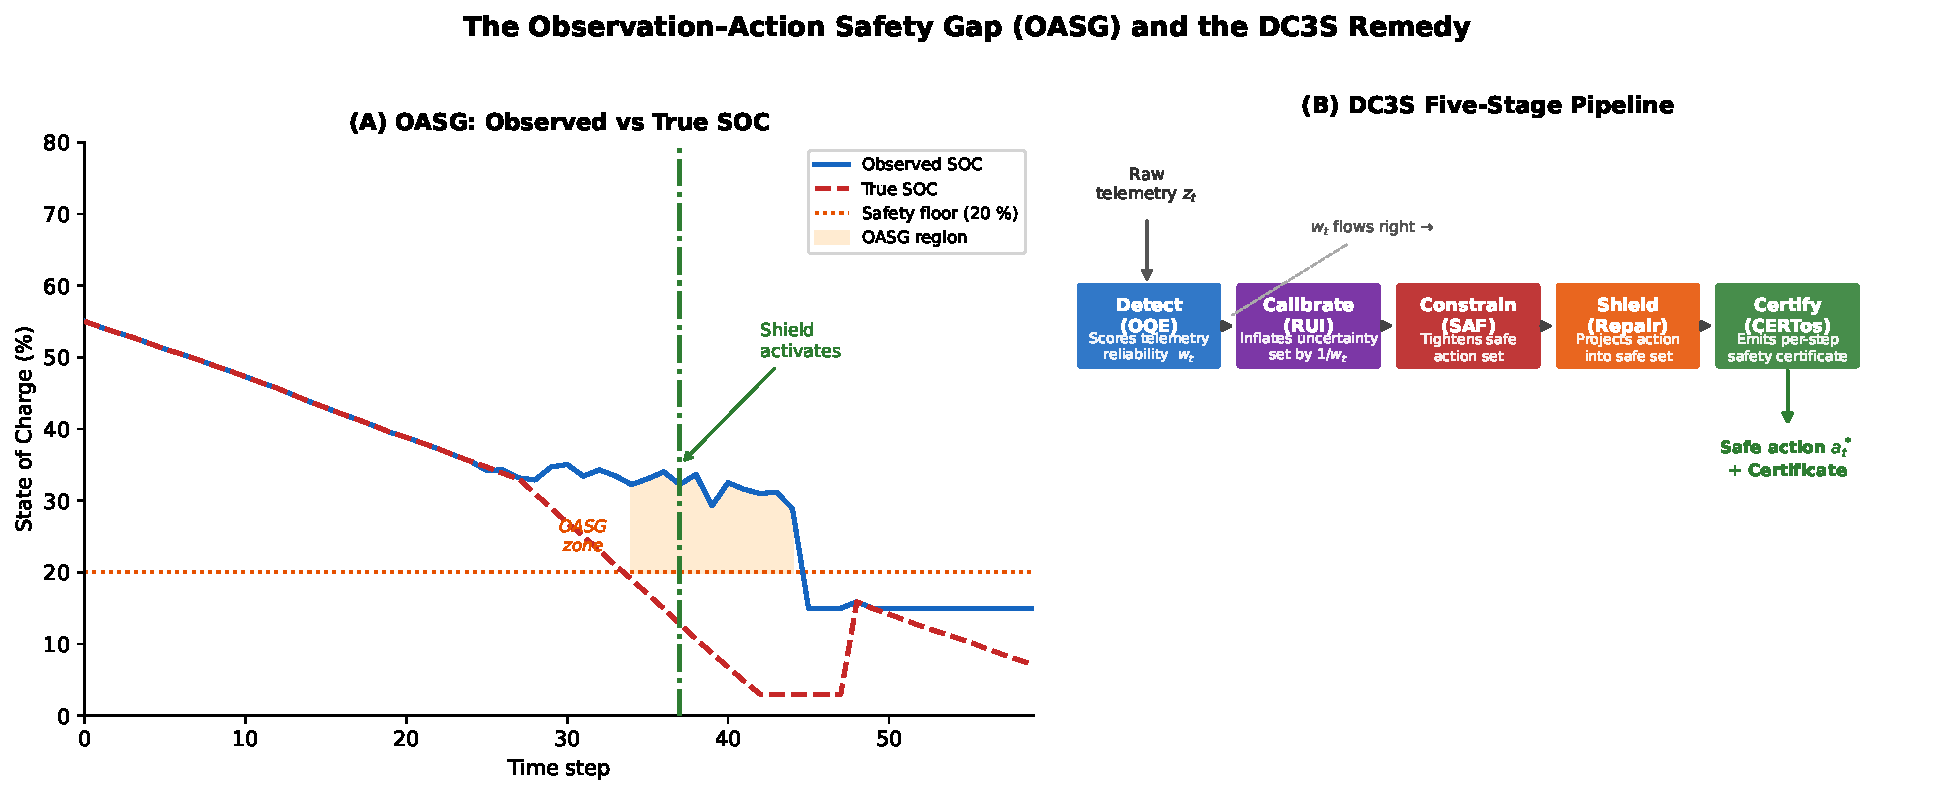
\includegraphics[width=\linewidth]{fig_oasg_hero}
\caption{Degraded observation turns controller legality into a latent safety hazard:
the candidate action can be valid on the observed state while unsafe on the true state.}
\label{fig:prof-oasg}
\end{figure}

ORIUS turns this hazard into a runtime object by making observation quality explicit.
Let \(w_t \in [0,1]\) be a reliability score computed from freshness, missingness,
sensor disagreement, residual behavior, or domain-specific degradation signatures. The
observation-consistent set is then inflated as
\begin{equation}
  U_t
  =
  \left\{
    x \in \mathcal{X} :
    d_t(x,\hat{x}_t) \le \beta_0 + \lambda(1-w_t) + \delta_t
  \right\},
\end{equation}
where \(\beta_0\) is the nominal uncertainty radius, \(\lambda(1-w_t)\) is the
reliability-conditioned inflation, and \(\delta_t\) captures drift- or history-based
correction. The universal contract does not insist on a single metric \(d_t\); it
insists only that the set widens monotonically when reliability falls.

The corresponding tightened safe-action set is
\begin{equation}
  \mathcal{A}^{\mathrm{safe}}_t(U_t)
  =
  \left\{
    a \in \mathcal{A} :
    g(x,a) \le 0,\ \forall x \in U_t
  \right\},
\end{equation}
where \(g(x,a)\) is the domain safety constraint. The released action is then
\begin{equation}
  a_t^{\mathrm{safe}}
  =
  \begin{cases}
    a_t^{\mathrm{cand}}, & a_t^{\mathrm{cand}} \in \mathcal{A}^{\mathrm{safe}}_t(U_t), \\
    \mathcal{R}_t(a_t^{\mathrm{cand}}, \mathcal{A}^{\mathrm{safe}}_t(U_t)), &
      \mathcal{A}^{\mathrm{safe}}_t(U_t) \neq \varnothing, \\
    \mathcal{F}_t(c_t), & \mathcal{A}^{\mathrm{safe}}_t(U_t) = \varnothing,
  \end{cases}
\end{equation}
with repair map \(\mathcal{R}_t\), fallback policy \(\mathcal{F}_t\), and certificate
context \(c_t\).

This yields the central runtime question for the paper: once degraded observation is
acknowledged, what set of actions remains certifiably safe and auditable? ORIUS answers
that question with one runtime kernel, one benchmark schema, and one governance
discipline. The theorem bridge later shows that the resulting safety layer is not a
heuristic wrapper but a structured bound-preserving construction under explicit
assumptions.

\section{Related Work and the Insufficiency of Prior Families}
\label{sec:prof-related-work}

ORIUS does not claim that prior work ignored uncertainty or safety. The claim is
narrower and stronger: the major adjacent families solve pieces of the problem, but not
the full runtime bridge from degraded observation to repaired actuation and auditable
release.

\subsection{Conformal prediction and calibration are necessary, but not enough}
Distribution-free and conformal methods provide finite-sample uncertainty surfaces for
learned predictors \cite{vovk2005algorithmic,lei2018distribution,romano2019conformalized,gibbs2021adaptive,zaffran2022adaptive,angelopoulos2023gentle,barber2023beyond}.
These tools are indispensable for ORIUS because the runtime must widen the
observation-consistent set when reliability drops. But they do not, by themselves,
specify which action remains legal after that widening. A prediction interval is not a
certificate of actuation legality. ORIUS therefore treats calibration as the input to a
safety layer rather than as the safety layer itself.

\subsection{Runtime assurance and Simplex-style supervision do not close the observation gap}
Runtime assurance, supervisory control, and Simplex-style architectures
\cite{sha1998simplex,sha2001using,desai2019soter,bloem2015shield,bartocci2018introduction,leucker2009brief,havelund2004runtime}
show that nominal intelligence should not be the final authority over actuation. ORIUS
inherits that insight directly. The gap is that many supervisory designs begin after a
candidate action already exists and assume that the state estimate is coherent enough to
be monitored. ORIUS starts earlier: it treats the observation surface itself as unsafe,
which forces the runtime to reason jointly about reliability, uncertainty inflation,
repair geometry, fallback, and certificate validity.

\subsection{Safety filters and constrained control are mathematically strong but plant-local}
Barrier functions, robust MPC, tube MPC, predictive safety filters, and reachability-
based controllers can turn model uncertainty into admissible action sets
\cite{ames2014cbf,ames2019control,wabersich2021predictive,fisac2019general,mayne2005robust,langson2004tubes,camacho2013model,rawlings2017mpc}.
ORIUS does not compete with that mathematics. It packages those ideas behind a typed
runtime contract that can host multiple geometries across multiple plants. The
scientific move is not a new universal controller; it is one reusable way to make
degraded observation alter actuation semantics.

\subsection{Anomaly, drift, and fault detection stop too early}
Change detection, drift detection, anomaly scoring, and CPS fault analysis provide the
language for recognizing when telemetry should no longer be trusted
\cite{basseville1993detection,page1954continuous,page1955test,hinkley1971inference,breunig2000lof,liu2008isolation,pasqualetti2013attack,teixeira2015secure}.
Yet many systems stop at an alarm or a reliability score. ORIUS treats that as an
incomplete runtime response. Once trust has fallen, the system still needs to decide
which actions remain legal, which actions must be repaired, when fallback is required,
and how that decision is certified.

\subsection{Domain-specific safety work rarely becomes a universal runtime grammar}
Energy dispatch, autonomous driving, clinical monitoring, and other physical-AI safety
settings each contain strong plant-level ideas, but most remain
tied to one domain's state geometry, one benchmark, and one intervention semantics. The
result is local excellence without a shared runtime object. ORIUS positions itself as a
cross-domain safety-layer grammar that can sit above those domain-specific methods while
keeping the data and proof posture explicitly tiered.

\begin{table*}[t]
\centering
\small
\caption{Why prior families remain necessary but insufficient for the ORIUS object.}
\label{tab:prof-family-gap}
\begin{tabularx}{\textwidth}{@{}p{0.17\textwidth}p{0.25\textwidth}p{0.50\textwidth}@{}}
\toprule
\textbf{Method family} & \textbf{What it contributes} & \textbf{Why it is insufficient for OASG} \\
\midrule
Conformal and adaptive calibration & Distribution-free uncertainty and shift-aware coverage control & Does not decide repaired actuation, fallback legality, or certificate release after trust degrades. \\
Runtime assurance and shielding & Supervisory interception and safety-controller fallback & Often assumes the observation surface is coherent enough to supervise directly. \\
Safety filters and robust constrained control & Strong admissible-set mathematics under uncertainty & Usually remains plant-local and does not define a reusable benchmark/governance contract. \\
Anomaly, drift, and fault detection & Detects that telemetry has become unreliable & Stops at alarms or scores unless paired with repair, fallback, and audit semantics. \\
Domain-specific CPS safety stacks & High-quality local solutions in one plant family & Rarely expose a universal runtime grammar that transfers across domains without changing the scientific object. \\
\bottomrule
\end{tabularx}
\end{table*}

The ORIUS thesis is therefore integrative but not vague. The universal object is not
``safe AI'' in the abstract. It is the typed runtime layer that binds reliability,
uncertainty, admissible actions, repaired release, and certificate governance under one
action-semantics problem.

\section{ORIUS Runtime Architecture}
\label{sec:prof-runtime-architecture}

ORIUS is a post-nominal runtime layer. It does not replace the upstream predictor,
planner, optimizer, or policy. It wraps them with a narrow contract that begins at raw
telemetry and ends at certificate-gated release. This is the architectural reason the
framework can remain domain-agnostic even when the domains do not share nominal models
or action geometry.

\begin{figure*}[t]
\centering
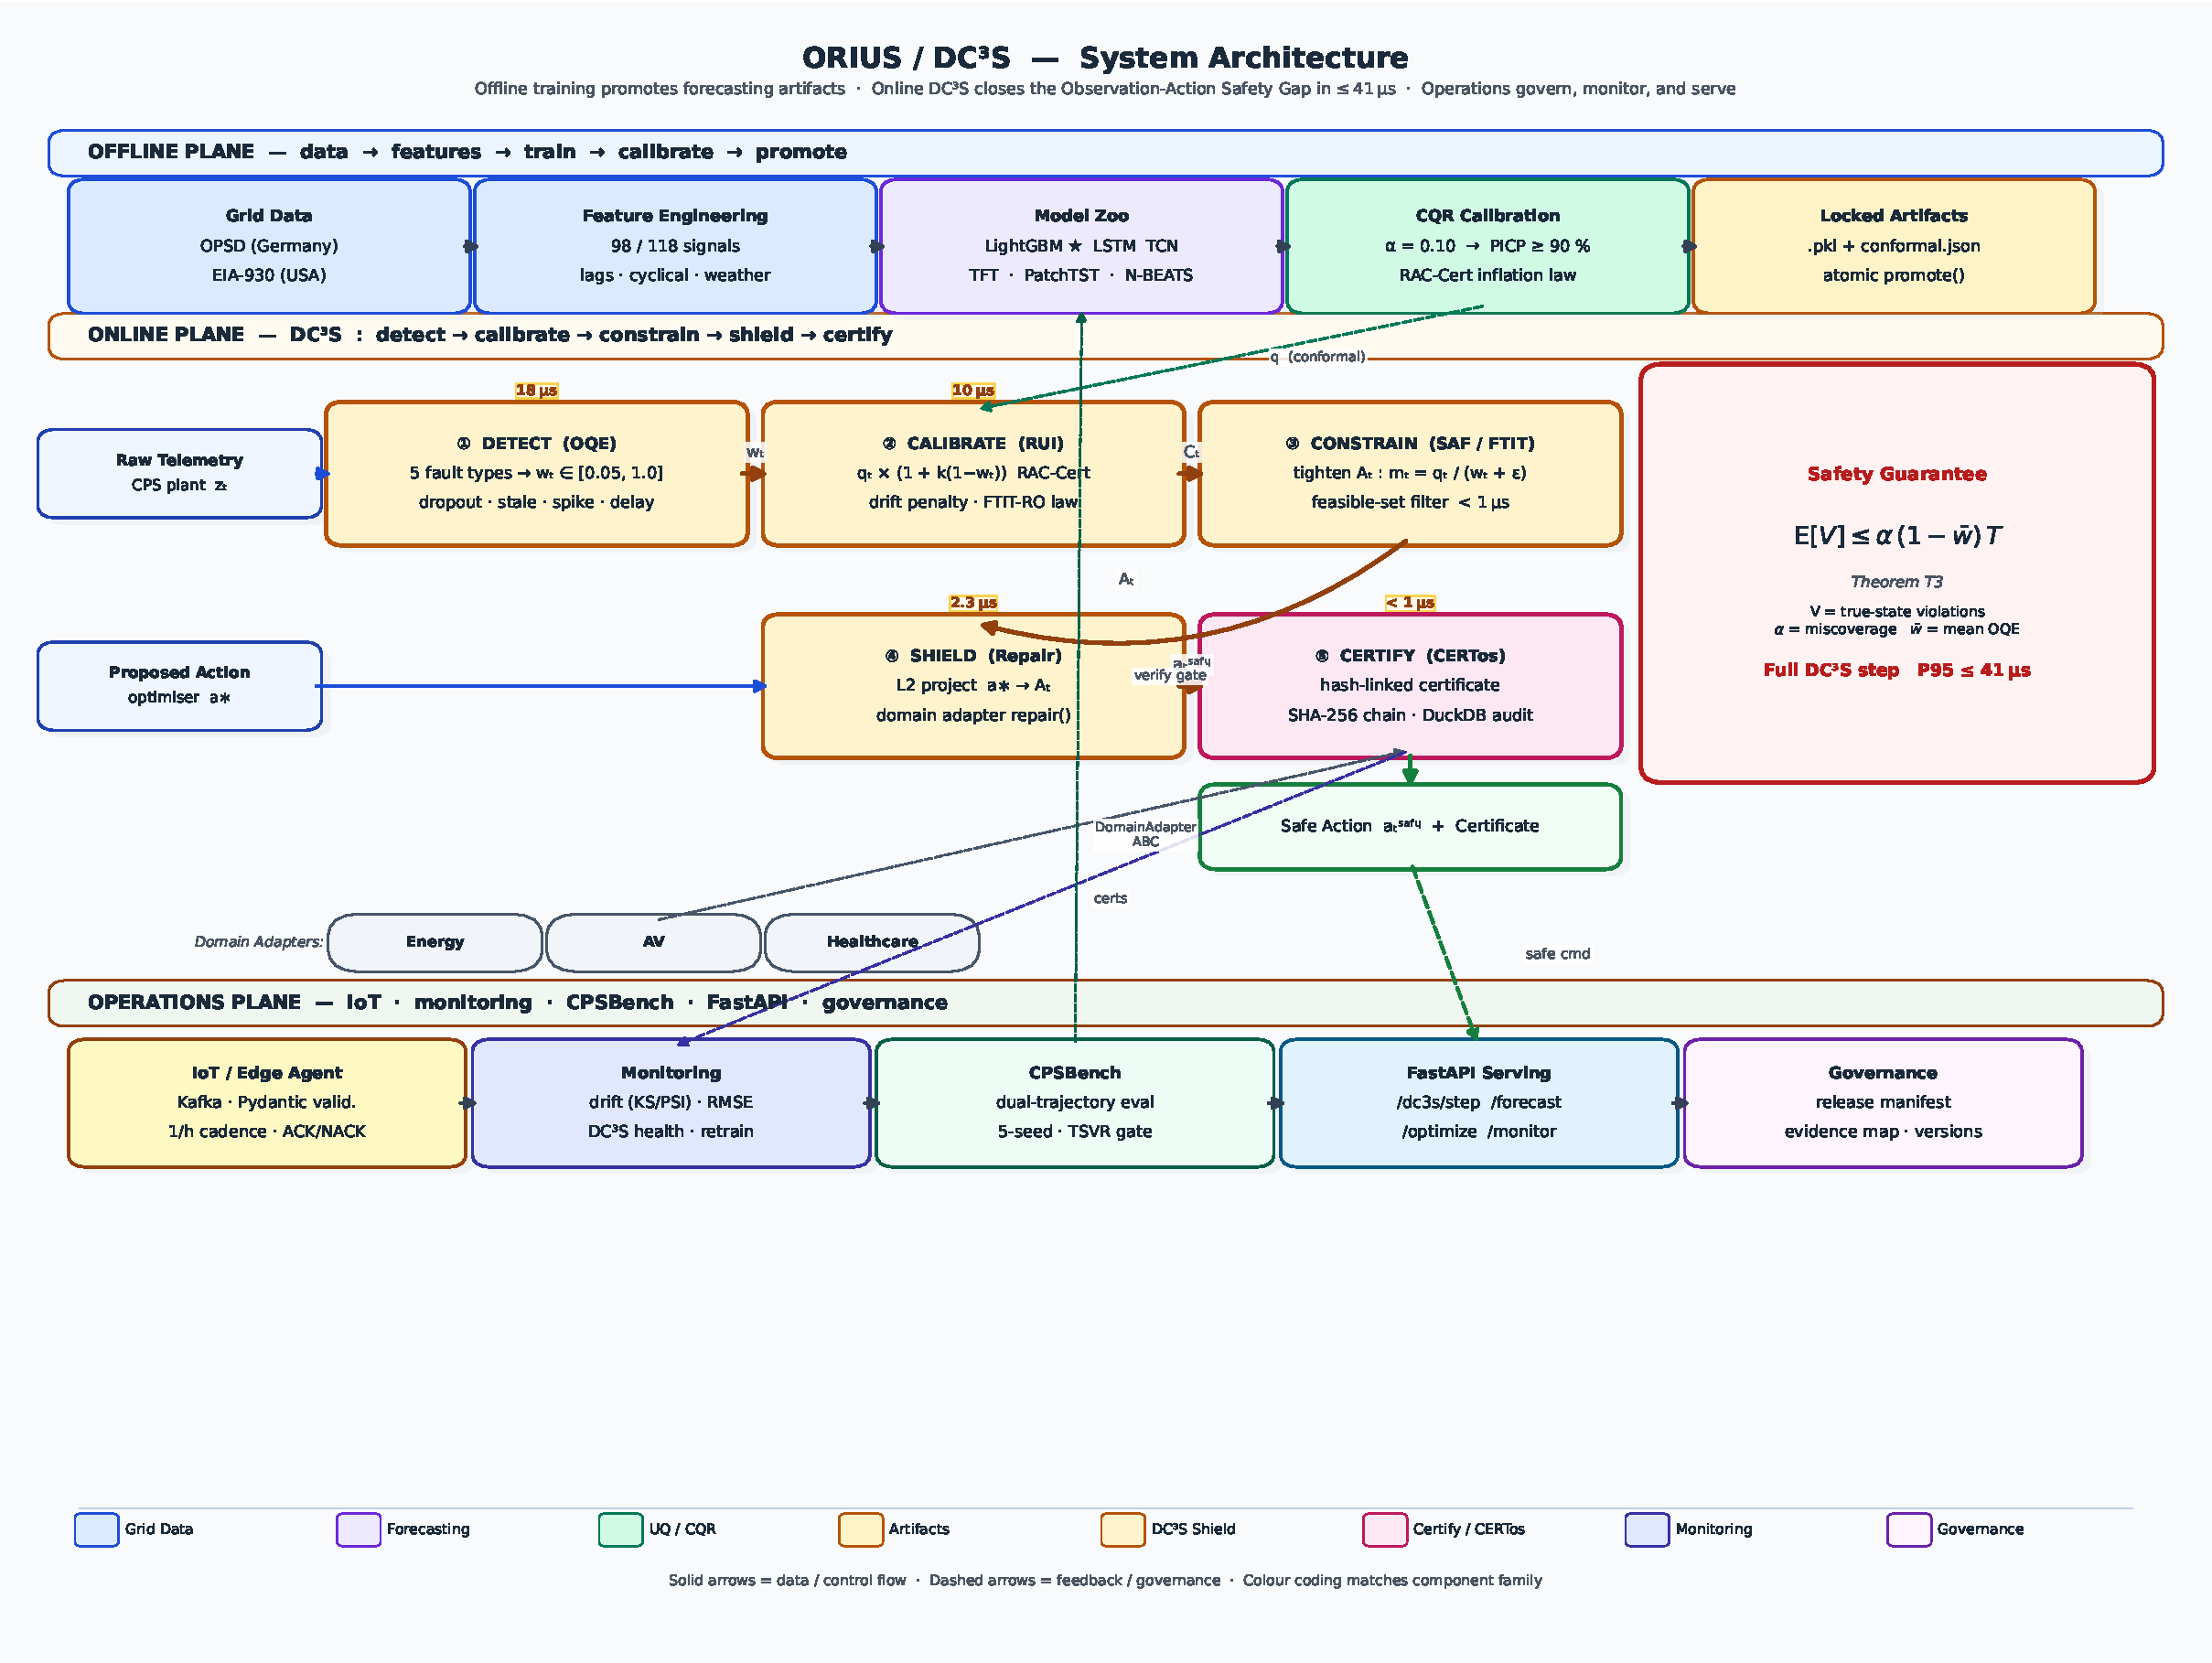
\includegraphics[width=0.95\textwidth]{fig01_architecture}
\caption{ORIUS as a universal runtime layer between nominal intelligence and physical
actuation. Domain-specific adapters feed a shared Detect--Calibrate--Constrain--Shield--
Certify kernel whose outputs are benchmarked and governed under one contract.}
\label{fig:prof-architecture}
\end{figure*}

The kernel consists of five stages.
\begin{enumerate}[leftmargin=1.25em,itemsep=0.2em]
  \item \textbf{Detect:} estimate reliability \(w_t\) and drift flags from freshness,
  missingness, cross-sensor consistency, residual behavior, and domain-specific
  diagnostics.
  \item \textbf{Calibrate:} inflate the observation-consistent set \(U_t\) rather than
  trusting a nominal point estimate.
  \item \textbf{Constrain:} recompute the safe action set under the widened state set.
  \item \textbf{Shield:} keep, repair, or replace the candidate action.
  \item \textbf{Certify:} emit a causal certificate and update the governance state.
\end{enumerate}

The kernel becomes scientific rather than architectural once its objects are written
explicitly. ORIUS uses a reliability-conditioned uncertainty envelope
\begin{equation}
  U_t
  =
  \left\{
    x :
    m_t(x,\hat{x}_t) \le q_{1-\alpha_t}(w_t,\Delta_t)
  \right\},
\end{equation}
where \(m_t\) is a domain-specific mismatch measure and \(q_{1-\alpha_t}\) is a
reliability-aware quantile or inflation operator. The tightened action set is
\begin{equation}
  \mathcal{A}^{\mathrm{safe}}_t(U_t)
  =
  \{a \in \mathcal{A}: g(x,a)\le 0,\ \forall x \in U_t\},
\end{equation}
and the certificate-relevant margin is
\begin{equation}
  \gamma_t(a)
  =
  \inf_{x \in U_t} \phi\!\bigl(f(x,a,0)\bigr),
\end{equation}
so that \(\gamma_t(a) \ge 0\) indicates one-step safety for every state in the
observation-consistent set.

\begin{algorithm}[t]
\caption{Detect--Calibrate--Constrain--Shield--Certify Runtime Step}
\label{alg:prof-runtime-step}
\begin{algorithmic}[1]
\Require observation packet \(o_t\), history \(\mathcal{H}_t\), candidate action
\(a_t^{\mathrm{cand}}\)
\State compute reliability score \(w_t\) and degradation flags from \(o_t\)
\State build observation-consistent set \(U_t\) using reliability-aware inflation
\State construct tightened safe-action set \(\mathcal{A}^{\mathrm{safe}}_t(U_t)\)
\If{\(a_t^{\mathrm{cand}} \in \mathcal{A}^{\mathrm{safe}}_t(U_t)\)}
  \State \(a_t^{\mathrm{safe}} \gets a_t^{\mathrm{cand}}\)
\ElsIf{\(\mathcal{A}^{\mathrm{safe}}_t(U_t) \neq \varnothing\)}
  \State \(a_t^{\mathrm{safe}} \gets \mathcal{R}_t(a_t^{\mathrm{cand}}, \mathcal{A}^{\mathrm{safe}}_t(U_t))\)
\Else
  \State \(a_t^{\mathrm{safe}} \gets \mathcal{F}_t(c_t)\)
\EndIf
\State emit certificate \(c_t\) with \((w_t,U_t,\gamma_t,\texttt{mode},\texttt{audit\_hash})\)
\State release \(a_t^{\mathrm{safe}}\) only if certificate is valid or fallback is explicit
\end{algorithmic}
\end{algorithm}

This algorithm is the real reusable object in ORIUS. It explains why the framework can
support batteries, vehicles, industrial plants, healthcare monitoring, navigation, and
aerospace without pretending those domains share the same nominal control law. What is
shared is the runtime grammar that mediates degraded observation before actuation.

\section{Universal Contracts: Adapter, Benchmark, and CertOS Governance}
\label{sec:prof-runtime-contracts}

The professor-facing ORIUS draft should present three contracts as a single
stack: the adapter contract, the benchmark contract, and the CertOS
governance contract.  Together they explain how degraded observation is
converted into a typed runtime safety layer rather than a battery-only
control recipe.

\subsection{Adapter contract}
The adapter is the only place where domain-specific telemetry and
constraints are allowed to enter the universal runtime.  The current
monograph and supporting design documents make this boundary explicit:
\texttt{src/orius/certos/runtime.py} provides a domain-neutral governance
surface, \texttt{docs/UNIVERSAL\_BENCHMARK\_SPEC.md} defines the common
step schema, and \texttt{docs/UNIVERSAL\_GOVERNANCE\_SPEC.md} requires a
domain governance policy instead of battery-shaped runtime state.

In practical terms, each domain adapter must expose a true-state violation
predicate, an observed-state satisfiability predicate, an optional margin
computation, a fallback action, and certificate-compatible action repair.
That is the minimum needed to make ORIUS portable across battery energy
storage, autonomous vehicles, industrial control, healthcare monitoring,
navigation, and aerospace without changing the meaning of safety at the
kernel level.

\subsection{Benchmark contract}
ORIUS-Bench is the manuscript-facing replay contract. The universal step
record keeps the same fields across domains:
\texttt{true\_constraint\_violated},
\texttt{observed\_constraint\_satisfied},
\texttt{true\_margin},
\texttt{observed\_margin},
\texttt{intervened},
\texttt{fallback\_used},
\texttt{certificate\_valid},
\texttt{latency\_us}, and
\texttt{domain\_metrics}. The metrics family is equally fixed: TSVR, OASG,
certificate validity accuracy, intervention rate, audit completeness,
latency percentiles, and coverage diagnostics when conformal uncertainty is
active.

This contract matters because it prevents the professor-facing draft from
collapsing the whole manuscript into a single battery result table.  It
also keeps the evidence boundary honest: the same schema can be reused
across all six rows, but the rows do not carry the same proof depth.

\subsection{CertOS governance contract}
CertOS is the runtime governance layer.  Its role is deliberately narrow:
do not release an action unless the runtime can either validate a current
certificate or replace the action with an explicit fallback.  The policy
surface is domain-neutral and consists of five hooks:
\texttt{is\_actuation(action)},
\texttt{fallback\_action(constraints, state)},
\texttt{horizon\_update(certificate, reliability, drift, constraints, validity\_horizon)},
\texttt{required\_certificate\_fields()}, and
\texttt{integrity\_projection(action)}.

The invariants are correspondingly small and auditable: no actuation
without a valid or fallback certificate path, an unbroken certificate hash
chain, and fallback only when validity collapses. That is the right level
of abstraction for a professor-facing draft that wants to argue for a
fundamental safety layer.

\begin{algorithm}[t]
\caption{CertOS Certificate Release and Lifecycle Update}
\label{alg:prof-certos}
\begin{algorithmic}[1]
\Require repaired action \(a_t^{\mathrm{safe}}\), certificate candidate \(c_t\), reliability \(w_t\), constraints \(\kappa_t\)
\State project \(a_t^{\mathrm{safe}}\) through \texttt{integrity\_projection}
\If{\texttt{required\_certificate\_fields()} missing}
  \State mark certificate invalid and request fallback
\EndIf
\State validate lifecycle state and audit hash continuity
\If{certificate valid}
  \State compute horizon update using \texttt{horizon\_update}
  \State append validated certificate to audit ledger
  \State release projected action
\Else
  \State replace with \texttt{fallback\_action} and append degraded certificate
  \State release fallback only if lifecycle invariants still hold
\EndIf
\end{algorithmic}
\end{algorithm}

The professor-facing version should end this section with the claim
boundary stated plainly: ORIUS is a universal runtime safety contract for
Physical AI under degraded observation, but the evidence remains tiered by
domain and should not be presented as equal-depth proof across all rows.

\section{Theory Bridge and Promotion Discipline}
\label{sec:prof-theory-bridge}

This section distills the formal spine of ORIUS for a professor-facing IEEE draft.  It
connects the battery proof ladder, the universal kernel, and the cross-domain promotion
logic without reintroducing the full monograph narrative.  The key point is that ORIUS
is not presented as a battery theorem generalized by analogy.  It is presented as a
runtime safety grammar whose transfer obligations are explicit, checkable, and separate
from the evidence hierarchy.

\begin{figure}[t]
\centering

\includegraphics[width=\linewidth]{fig_orius_theory_runtime_domain_flow}
\caption{The theory bridge separates three levels of the claim: formal runtime objects,
domain-specific evidence obligations, and promotion status under the defended 3-domain discipline.}
\label{fig:prof-theory-runtime-domain}
\end{figure}

\subsection{Formal setting}
We consider a partially observed safety-constrained control system on a discrete
horizon \(t=0,1,\dots,T-1\):
\[
  x_{t+1}=f(x_t,a_t,\omega_t), \qquad
  y_t=h(x_t,\nu_t), \qquad
  w_t=\psi(y_{0:t}),
\]
with true state \(x_t\in\mathcal{X}\), action \(a_t\in\mathcal{A}\), observation
history \(\mathcal{H}_t=\sigma(y_{0:t})\), and reliability score \(w_t\in[0,1]\).
The safe set is
\[
  \mathcal{S}=\{x\in\mathcal{X}:\phi(x)\ge 0\},
\]
and the episode violation count is
\[
  V_T=\sum_{t=0}^{T-1}\mathbf{1}[x_t\notin\mathcal{S}].
\]
The ORIUS runtime layer takes a nominal candidate action
\(a_t^{\mathrm{cand}}=\pi_t(\mathcal{H}_t)\), constructs an observation-consistent
state set \(U_t\), tightens the admissible action set
\(\mathcal{A}_t^{\mathrm{safe}}(U_t)\), repairs or replaces the candidate action, and
emits a causal certificate.

\subsection{Promotion discipline}
The active ORIUS branch uses a promotion discipline rather than a flat universality gate. A
domain instantiation is not promoted by rhetorical similarity; it is promoted when it supplies:
\begin{enumerate}
  \item a declared observation model and a reproducible replay or experimental protocol;
  \item a sound observation-consistent set \(U_t\) and a domain-specific safe-action set;
  \item a repair or fallback operator that is measurable, causal, and certificate-backed;
  \item a benchmark compatible with the universal schema and a certificate that can be audited;
  \item a domain-specific safety reduction result that can be checked against the shared contract.
\end{enumerate}
This discipline rule is the manuscript's main safeguard: architecture may be universal
before evidence is broad, but the defended empirical claim remains limited to the
promoted three-domain lane until additional domains discharge the same obligations.
For theorem promotion specifically, status is governed by
\texttt{reports/publication/theorem\_promotion\_matrix.csv} and
\texttt{reports/publication/theorem\_result\_cards/*.json}.  The dashboard and
manuscript may call a row flagship only when the statement, assumptions, proof,
code anchor, tests, artifacts, hashes, manuscript anchor, and claim-boundary note
are all present.

\begin{proposition}[Promotion discipline]
\label{prop:universality-gate}
If a domain instantiation satisfies the universal adapter contract and discharges the
promotion obligations above, then the ORIUS kernel can be interpreted on that domain as a
runtime safety layer with the same formal objects used in the battery reference proof:
observation reliability, uncertainty inflation, admissible repair, fallback, and
certificate semantics.  If those obligations are not discharged, the manuscript may
retain only a bounded or gated claim.
\end{proposition}

\begin{proof}[Proof sketch]
The proposition is a packaging statement, not a new control theorem.  It follows directly
from the typed kernel and adapter surface described in the universal-completeness chapter:
the runtime only requires an observation packet, a reliability score, an observation-
consistent state set, a tightened safe-action set, a repair operator, a fallback, and a
causal certificate.  Appendix~A lists these objects and their assumption dependencies.
Once a domain supplies the same objects, the formal language of the battery ladder applies
without changing the runtime contract; what changes is the evidence status of the domain.
\end{proof}

\subsection{T5--T7\_Battery: Temporal certificate and fallback support}
Certificates are temporal objects. T5 (Finite-Horizon Certificate Validity) is a
flagship finite-horizon theorem: if the reachable tube from the
observation-consistent state set stays inside the safe set through horizon~$h$,
the certificate remains valid through that horizon unless invalidating evidence
arrives. T6 (Certificate Expiration Bound) adds a confidence-aware
closed-form first-passage lower-bound proposition on the remaining certificate
life, using the current boundary gap and the drift proxy $\sigma_d$.
T7\_Battery (Feasible Fallback Existence) then closes the operational loop as a
supporting proposition with a piecewise battery fallback: safe hold on the
interior, boundary-aware safe landing near the boundary, and fail-closed behavior
when neither case is certifiable. These surfaces are runtime-enforced:
when the T6 lower bound drops below one step, the guarantee check fails and the shield
must discharge the C7\_BatteryFallback contract.

\subsection{T9: Impossibility of quality-ignorant mandatory release}
T9 is promoted only in its scoped empty-safe-core form.  It is not a universal
claim about controllers allowed to abstain, expand uncertainty, fallback, or deny
release.

The first lower-bound claim is that ignoring reliability is not a benign
simplification when the observation class hides latent states with disjoint safe
actions.

\begin{theorem}[T9: Impossibility of quality-ignorant mandatory release]
\label{thm:prof-t9}
For an observation \(o\), let \(B(o)=\{x:h(x)=o\}\) and
\(K(o)=\cap_{x\in B(o)}C(x)\). If \(B(o)\ne\varnothing\) and
\(K(o)=\varnothing\), no total observation-only mandatory-release controller
can guarantee true-state safety for every \(x\in B(o)\).
\end{theorem}

\begin{proof}[Proof sketch]
The controller must choose one action \(a=\pi(o)\) for the nonempty ambiguity
class. Empty common safe core means no single action belongs to all \(C(x)\) for
\(x\in B(o)\), so some latent state in the ambiguity class makes that mandatory
release unsafe.
\end{proof}

\subsection{T10: Boundary-indistinguishability lower bound}
T10 is a two-state lower-bound theorem.  It does not claim a global minimax
frontier or matching optimality result.

\begin{theorem}[T10: Boundary-indistinguishability lower bound]
\label{thm:prof-t10}
Let \(x_0,x_1\) be boundary states with observation laws \(P_0,P_1\). If
\(d_{\mathrm{TV}}(P_0,P_1)\le\epsilon\) and
\(C(x_0)\cap C(x_1)=\varnothing\), then every observation-only
mandatory-release controller satisfies
\[
  \sup_{i\in\{0,1\}}\Pr_{O\sim P_i}[\pi(O)\notin C(x_i)]
  \ge \frac{1-\epsilon}{2}.
\]
\end{theorem}

\begin{proof}[Proof sketch]
This is a Le Cam style reduction.  For a deterministic release rule, let
\(S_i=\{o:\pi(o)\in C(x_i)\}\).  Disjoint safe-action sets imply
\(S_0\cap S_1=\varnothing\).  A test that decides \(x_0\) on \(S_0\) and
\(x_1\) otherwise succeeds at least as often as the release rule is safe, so the
two-point testing limit \((1+d_{\mathrm{TV}}(P_0,P_1))/2\) upper-bounds release
success.  The displayed lower bound follows by complementing and taking the
larger of the two state risks.  Randomized controllers follow by conditioning
on their internal seed.
\end{proof}

\subsection{Active theorem package after promotion}
The promoted theorem package is deliberately stronger than a relabeling exercise.  Each
surface now has a narrow mathematical statement, an explicit assumption footprint, a
proof source, a code anchor, tests, artifacts, and a claim-boundary note.  The result is
an active register with no defended draft rows.  T5 is a finite-horizon certificate
validity theorem rather than a definition-only row: the certificate is valid exactly
while the reachable tube remains inside the safe set and no invalidating evidence has
arrived.  T8 is a graceful-degradation dominance theorem only after adding useful work:
shutdown may be safe, but it does not satisfy the same safety--work partial order unless
it preserves the required operation fraction.  T9 and T10 are promoted as scoped
lower-bound results over observation-only mandatory release, not as unrestricted
statements about every possible runtime architecture.

The observation-robustness rows follow the same rule.  The Byzantine reliability result
is stated for a trimmed aggregation model with fewer than half corrupted channels; the
corollary to the ORIUS risk envelope is allowed only under that robust-score error
bound.  The stale-observation result is stated as bounded-drift uncertainty growth, not
as a physical law of geometric decay.  The runtime law suite is likewise narrow:
reliability-monotone inflation, safe-set antitonicity, intervention thresholding, and
the observation-ambiguity sandwich are small lemmas and propositions that support the
larger proof spine.  Tminimax is explicitly finite and scoped to two-state boundary
ambiguity classes, while the sensor-necessity row reduces missing critical coordinates
to the empty-safe-core condition.  These constraints are the reason the theorem package
can be ambitious without becoming overbroad.

\subsection{T11: Structural transfer through the universal adapter contract}
The third claim is the one that matters most for a universal paper draft.  It says that
the battery proof pattern can transfer if, and only if, the domain exposes the right
runtime objects.

\begin{theorem}[T11: Structural transfer]
\label{thm:prof-t11}
Let \(\mathcal{D}\) be any domain instantiation that satisfies the universal adapter
contract: it provides an observation packet, a reliability score \(w_t\), an
observation-consistent state set \(U_t\), a domain-safe action set
\(\mathcal{A}_t^{\mathrm{safe}}(U_t)\), a repair map, and a fallback action.  If
\(\Pr[x_t\in U_t\mid\mathcal{H}_t]\ge 1-\alpha\) and every repaired action lies in the
tightened safe-action set, then
\[
  \Pr[x_{t+1}\in\mathcal{S}\mid\mathcal{H}_t]\ge 1-\alpha.
\]
\end{theorem}

\begin{proof}[Proof sketch]
Condition on the observation history.  On the event \(x_t\in U_t\), soundness of the
tightened safe-action set implies that every admissible repaired action preserves the
safe set at the next step.  If the tightened set is empty, the fallback action preserves
safety by contract.  Therefore the only remaining source of failure is the probability
that the true state lies outside \(U_t\), which is at most \(\alpha\).  Appendix~A and
the theorem-surface register record the battery proof instances that instantiate this
logic in the reference domain.
\end{proof}

\begin{corollary}[Episode aggregation under a domain risk budget]
\label{cor:prof-episode-aggregation}
If a domain supplies a predictable per-step risk budget \(r_t\) such that
\(\Pr[x_{t+1}\notin\mathcal{S}\mid\mathcal{H}_t]\le r_t\), then
\[
  \mathbb{E}[V_T]\le \sum_{t=1}^T r_t.
\]
When the budget has the battery-style envelope \(r_t\le \alpha(1-w_t)\), the familiar
upper bound \(\mathbb{E}[V_T]\le \alpha(1-\bar{w})T\) follows immediately.
\end{corollary}

\subsection{Interpretation for the IEEE draft}
The practical message for the IEEE manuscript is that the theory bridge does not need to
be a second thesis chapter.  It needs to do three things well: state the universal
objects, state the universality gate, and state the proof skeleton that connects the
reference battery ladder to any new domain that clears the adapter contract.  That is the
strongest possible version of the claim without inventing unsupported empirical parity.

This is why the theory bridge belongs in the main paper instead of disappearing into a
supplement. The ORIUS claim is not merely that a benchmark improved. It is that
degraded observation changes the structure of what safe release means, and that the
runtime layer makes that change explicit in a way that can be proved, benchmarked, and
audited.

\section{Battery Witness Results}
\label{sec:prof-battery-results}

The battery domain remains the strongest empirical witness in ORIUS, but it is
best read as a witness rather than the conceptual center of the framework.  The
locked battery artifacts show a clear separation between \emph{controllers that
can detect and repair under degraded observation} and those that cannot.  That
separation matters more than any single cost number: the decisive result is
whether true-state violations disappear under telemetry faults.

Table~\ref{tab:prof-battery-summary} condenses the strongest locked battery
evidence.  The repair-aware ORIUS variants are the only methods in this slice
that simultaneously eliminate true-state violations and retain meaningful
coverage.  The deterministic LP and static interval baselines fail on that
first criterion, while the wrapped and FTIT variants preserve safety at the
price of modest intervention.

\begin{table}[t]
\centering
\small
\caption{Compact battery witness summary from locked publication artifacts.
TSVR is true-state violation rate; coverage is the 90\% predictive interval
coverage reported by the baseline audit.}
\label{tab:prof-battery-summary}
\begin{tabular}{lrrrr}
\toprule
\textbf{Controller} & \textbf{TSVR (\%)} & \textbf{Repair / IR (\%)} &
\textbf{Coverage} & \textbf{Mean width} \\
\midrule
ORIUS FTIT & 0.000 & 2.798 & 0.971627 & 3906.548 \\
ORIUS Wrapped & 0.000 & 0.000 & 0.884127 & 559.921 \\
Adaptive Conformal + Repair & 0.000 & 1.389 & 0.962500 & 2824.252 \\
Deterministic LP & 3.909 & 0.000 & 0.883333 & 503.131 \\
Robust Fixed Interval & 25.575 & 0.000 & 0.883333 & 503.131 \\
\bottomrule
\end{tabular}
\end{table}

Two points follow directly from the evidence.  First, the safety gain is
structural: once reliability-aware repair is enabled, the hidden violation rate
drops to zero across the battery witness package.  Second, the deep quality
model is not being used as a claim of forecasting superiority.  The deep OQE
summary is only mildly predictive of fault family (\texttt{fault\_auc} $=0.534$),
which is precisely why the framework treats quality scoring as a guardrail for
repair and certificate logic rather than as a standalone predictor.

Figure~\ref{fig:prof-battery-baselines} provides the visual counterpart to the
table: the battery witness is strongest where the repair-and-certify layer keeps
the true-state violation surface at zero while leaving the non-repair baselines
exposed.

\begin{figure}[t]
\centering
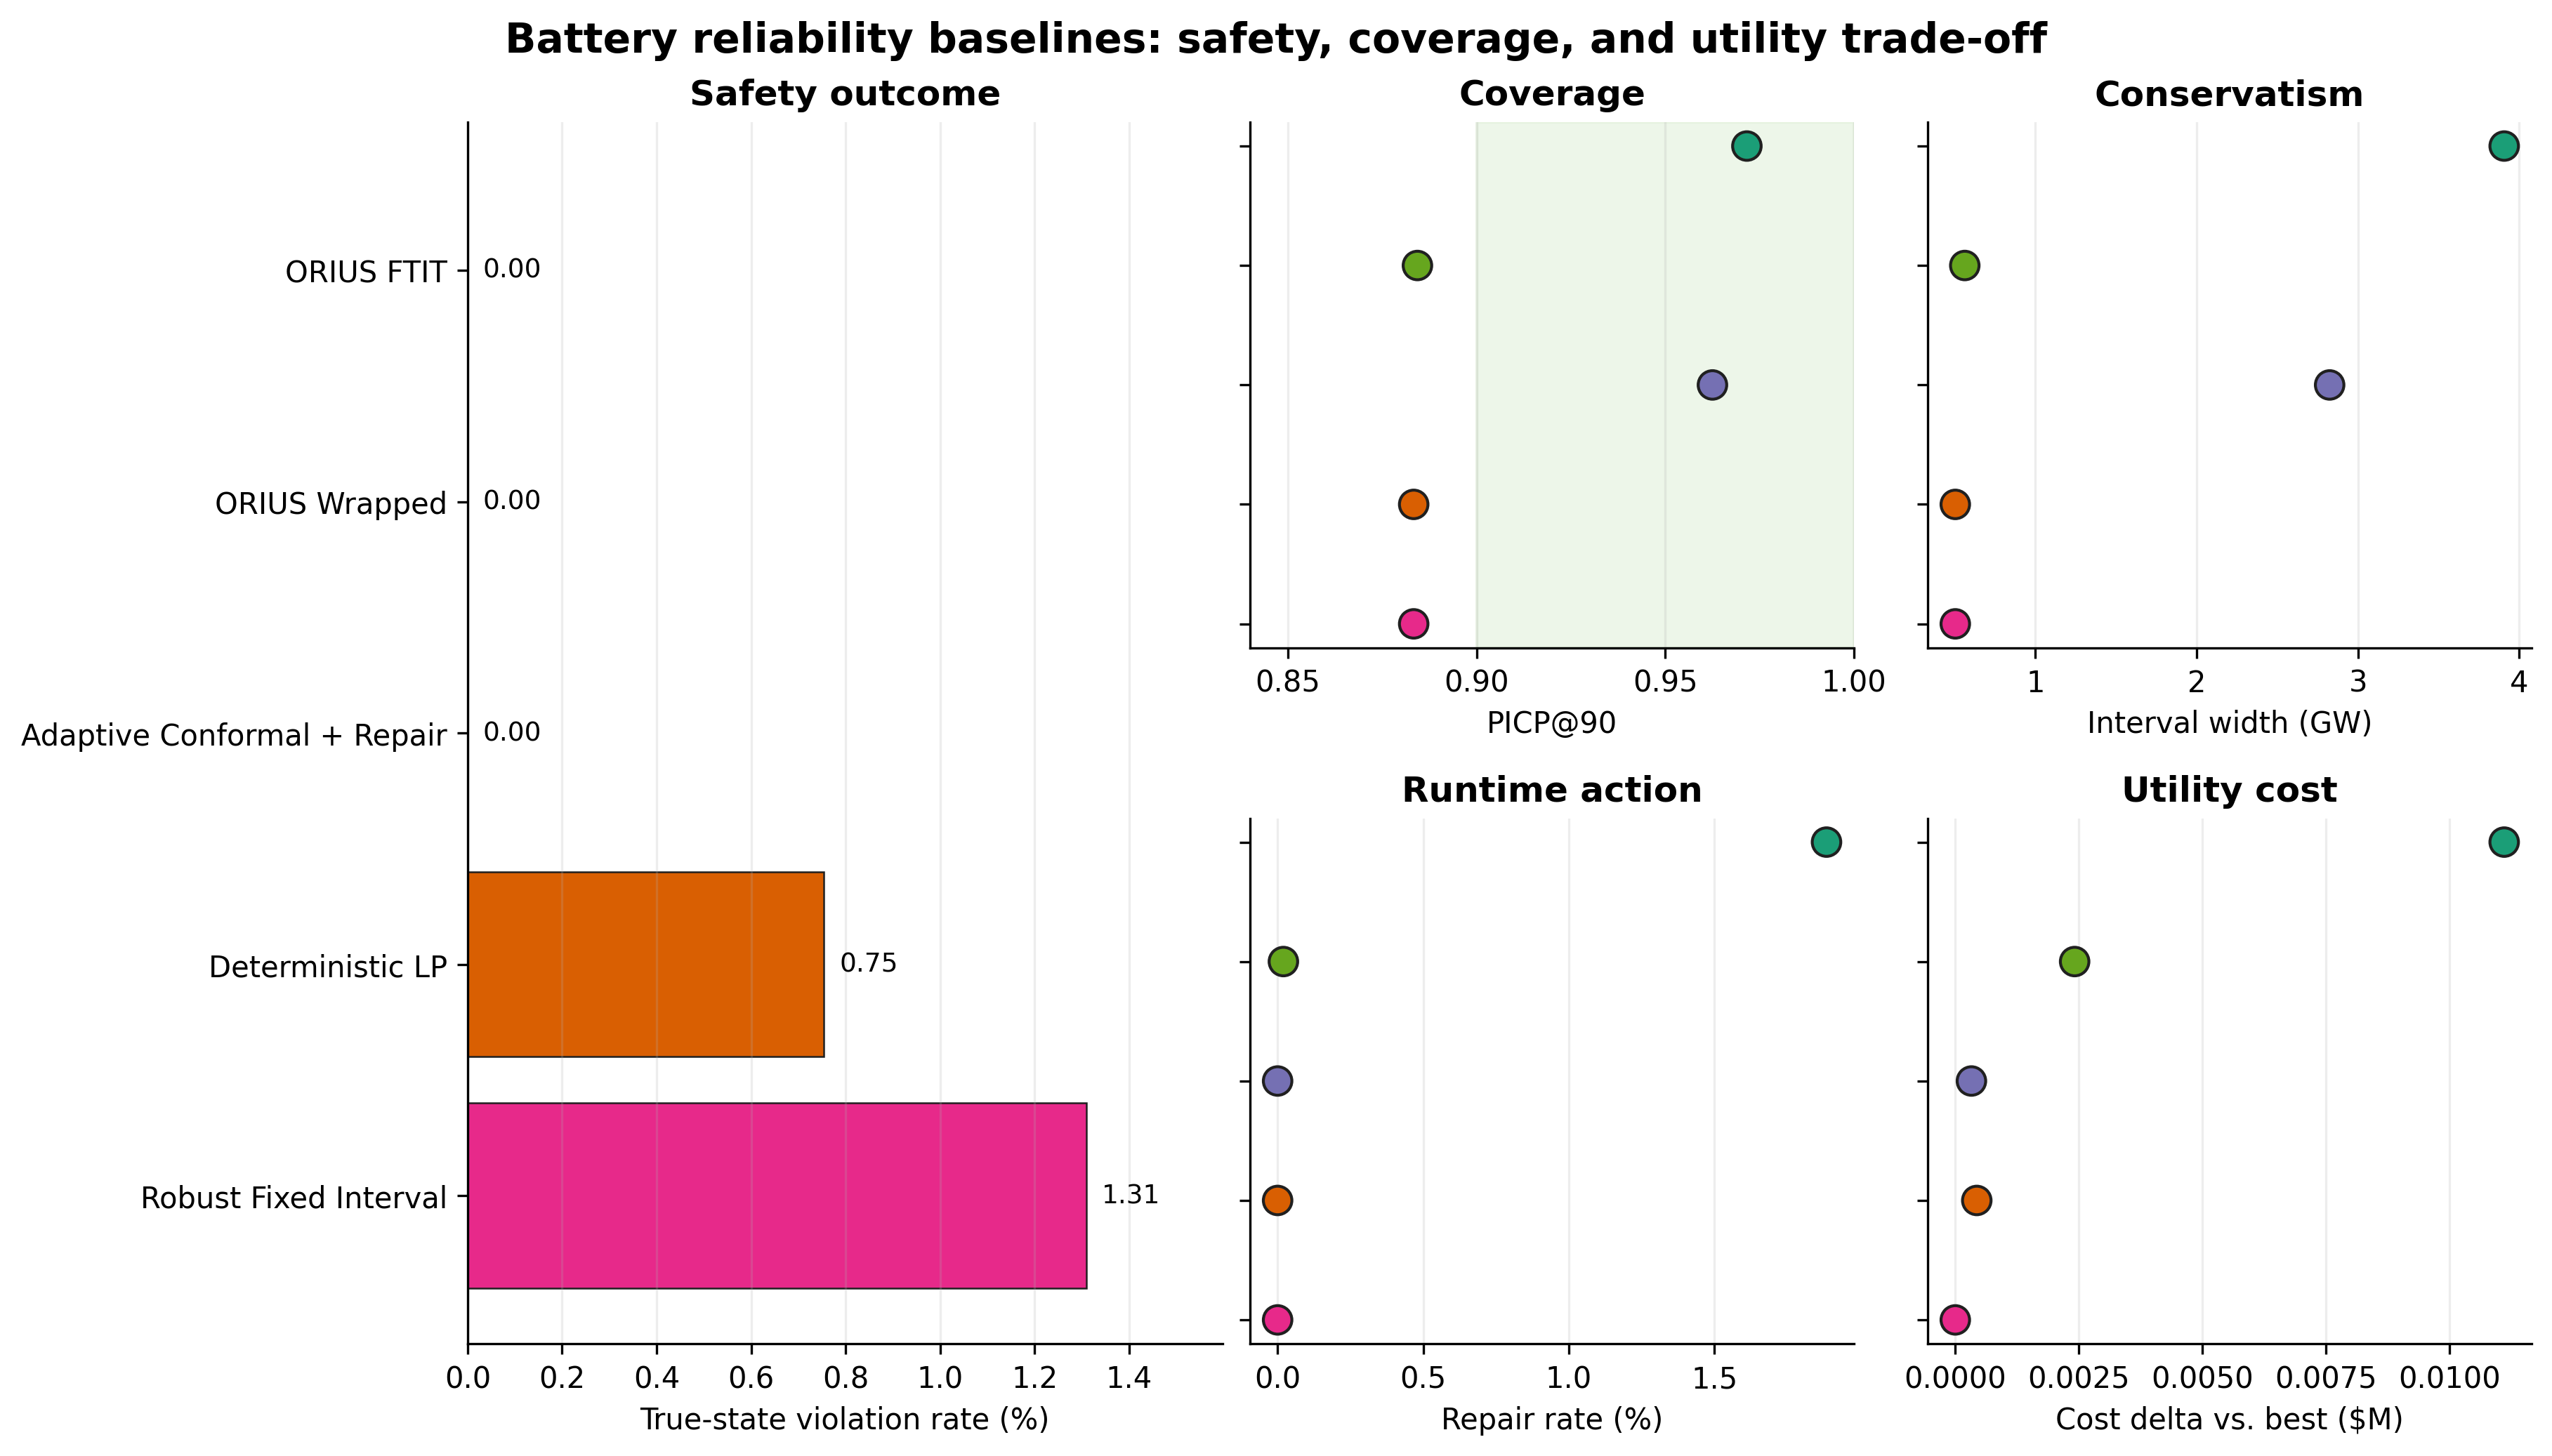
\includegraphics[width=\linewidth]{fig_battery_reliability_baselines}
\caption{Battery reliability baselines from the locked publication package.
The ORIUS repair-aware variants preserve zero true-state violations, while the
deterministic and static-interval baselines do not.}
\label{fig:prof-battery-baselines}
\end{figure}

The chapter-level battery results remain consistent with the publication
artifacts used elsewhere in the monograph: the locked controller comparison,
the reliability baseline audit, the 48-hour trace, and the ablation suite all
point to the same conclusion.  ORIUS is not merely reducing cost or widening
intervals; it is preventing hidden violations under observation degradation.

\paragraph{Bottom line.}
For a professor-facing ORIUS manuscript, this is the battery story worth
retaining in the main text: the battery plant is the cleanest empirical witness
that the observation-quality signal, repair step, and certificate discipline are
doing real work.  The detailed traces, fault-family responses, and ablations are
valuable, but they belong behind the compact result statement rather than
crowding it.

\section{Runtime and Empirical Results}
\label{sec:prof-results}

The decisive empirical question for ORIUS is not whether one domain achieves the lowest
cost or the smallest interval width. It is whether the runtime layer materially reduces
true-state violations under degraded observation while remaining operationally cheap and
auditable. The current repository truth supports that claim most strongly in the battery
witness row and then at bounded depth across AV, industrial, and healthcare.

The battery witness establishes the strongest result surface: ORIUS repair-aware
controllers eliminate true-state violations under the locked degraded-telemetry protocol
while maintaining bounded intervention rates. The cross-domain runtime evidence then
shows that the same runtime grammar remains cheap enough to be plausible across
non-energy domains. The important result is therefore joint: safety repair is doing real
work, and the added runtime layer is not computationally extravagant.

\begin{table*}[t]
\centering
\scriptsize
\caption{Runtime and governance summary for the professor-facing ORIUS draft.}
\label{tab:prof-runtime-governance}
\begin{tabularx}{\textwidth}{@{}p{0.24\textwidth}p{0.16\textwidth}p{0.14\textwidth}p{0.14\textwidth}p{0.12\textwidth}p{0.14\textwidth}@{}}
\toprule
\textbf{Domain} & \textbf{Row} & \textbf{P95 latency (ms)} & \textbf{Fallback (\%)} & \textbf{Audit / lifecycle (\%)} & \textbf{Boundary} \\
\midrule
Battery Energy Storage & Witness row & 0.812 & 100.0 & 100.0 & deepest theorem-to-artifact closure\\
Autonomous Vehicles & Defended bounded row & 0.744 & 100.0 & 100.0 & bounded TTC plus predictive-entry-barrier contract\\
Medical and Healthcare Monitoring & Defended bounded row & 0.701 & 100.0 & 100.0 & bounded monitoring and alert-release semantics\\
\bottomrule
\end{tabularx}
\end{table*}


Three results matter most.
\begin{enumerate}[leftmargin=1.25em,itemsep=0.2em]
  \item \textbf{Safety reduction:} the battery witness row is the clearest proof that
  reliability-conditioned repair prevents hidden violations that remain visible under
  deterministic and static-interval baselines.
  \item \textbf{Runtime plausibility:} the defended rows remain in the sub-millisecond
  regime at the P95 level, which means ORIUS behaves like a lightweight safety layer
  rather than a second controller.
  \item \textbf{Governed release:} certificates, fallback paths, and audit continuity
  are observed rather than assumed, so runtime safety is measured as a released-action
  discipline instead of an undocumented filter.
\end{enumerate}

The combined runtime-governance table also makes the evidence boundary easy to read.
Battery is the witness row. AV, industrial, and healthcare are defended bounded rows
with full certificate rates and bounded runtime semantics. Navigation and aerospace are
present in the runtime surface, but they remain blocked from defended closure for data
and task reasons rather than architecture reasons. That is exactly the disciplined claim
shape a professor-facing draft should preserve.

What this means scientifically is that ORIUS is being evaluated as a release layer, not
as a task policy. The battery witness demonstrates the deepest theorem-to-runtime
closure, but the runtime-governance table shows the more general point: intervention,
fallback, latency, and certificate validity can be measured under one contract across
qualitatively different physical systems. That is why the paper uses bounded rows and a
witness row rather than forcing every domain into one artificial leaderboard.

\begin{table*}[htbp]
\centering
\scriptsize
\caption{Deployment validation scope for the active three-domain ORIUS draft.}
\label{tab:orius-deployment-validation-scope}
\resizebox{\textwidth}{!}{%
\begin{tabular}{p{2.5cm}p{2.5cm}p{2.2cm}p{2.2cm}p{2.8cm}p{3.0cm}}
\toprule
\textbf{Deployment surface} & \textbf{Governing artifact} & \textbf{Scope type} & \textbf{Current status} & \textbf{Bounded manuscript claim} & \textbf{Exact non-claim or gap}\\
\midrule
Battery witness runtime & reports/publication/dc3s\_main\_table.csv & witness\_replay & bounded\_reference & Battery supports the deepest runtime and theorem witness surface. & This is still not unrestricted field deployment.\\
Autonomous-vehicle defended replay & reports/orius\_av/full\_corpus/runtime\_summary.csv & bounded\_replay & defended\_bounded & AV supports bounded replay under the TTC plus predictive-entry-barrier contract. & It does not claim full autonomous-driving closure.\\
Healthcare defended replay & reports/healthcare/runtime\_governance\_summary.csv & bounded\_replay & defended\_bounded & Healthcare supports bounded monitoring and alert-release claims. & It does not claim regulated clinical deployment and still uses governance-pass proxy wording for certificate-valid release.\\
OOD and adversarial completeness & chapters/ch34\_outside\_current\_evidence.tex; reports/publication/adversarial\_probing\_robustness\_table.csv & explicit\_non\_claim\_register & bounded\_non\_claim & The monograph can discuss bounded active probing and non-claim discipline. & It does not claim universal adversarial completeness or unrestricted OOD safety.\\
\bottomrule
\end{tabular}}
\end{table*}


The deployment-scope table prevents the results section from sliding into unbounded
deployment rhetoric. Even the strongest battery row stops short of unrestricted field
deployment. The defended bounded rows stop at replay-backed and runtime-governed
validation. The blocked rows remain visible precisely so that the paper's universal
architecture claim stays larger than a single benchmark number but smaller than a
universal deployment claim.

One further interpretive point matters for the professor review draft. ORIUS is not
claiming that every domain should optimize the same surface metric. Some rows care about
dispatch legality, others about headway or envelope preservation, others about
intervention legality. The universal result is instead that each domain can expose a
true-state safety object, and that ORIUS can reduce risk on that object by governing
release under degraded observation. That is the empirical thesis the paper can defend
without overstating parity.

\section{Cross-Domain Synthesis}
\label{sec:prof-cross-domain}

ORIUS is best read as a universal runtime safety layer for Physical AI, not as a
single-domain controller that happens to generalize.  The common object across the
monograph is the degraded-observation hazard: the controller sees an observation
surface, but safety is judged on the true state or the observation-consistent
state set.  That is why the same runtime grammar recurs across battery storage,
autonomous vehicles, industrial process control, healthcare monitoring, navigation,
and aerospace.

\begin{table*}[t]
\centering
\small
\caption{Cross-domain parity and promotion status for the professor-facing ORIUS draft.}
\label{tab:prof-cross-domain-status}
\begin{tabularx}{\textwidth}{@{}p{0.18\textwidth}p{0.18\textwidth}p{0.27\textwidth}p{0.27\textwidth}@{}}
\toprule
\textbf{Domain} & \textbf{Current row} & \textbf{What is currently closed} & \textbf{Current blocker or boundary} \\
\midrule
Battery Energy Storage & Witness row & adapter, replay, CertOS, soundness & battery\_reference\_witness\\
Autonomous Vehicles & Defended bounded row & adapter, replay, CertOS, soundness & promoted\\
Industrial Process Control & Defended bounded row & adapter, replay, CertOS, soundness & industrial\_train\_validation\_chain\_complete\\
Medical and Healthcare Monitoring & Defended bounded row & adapter, replay, CertOS, soundness & healthcare\_train\_validation\_chain\_complete\\
Navigation and Guidance & Shadow-synthetic & adapter, replay & navigation\_real\_data\_gap\\
Aerospace Control & Experimental & adapter, replay & aerospace\_experimental\_placeholder\\
\bottomrule
\end{tabularx}
\end{table*}


\begin{figure*}[t]
\centering
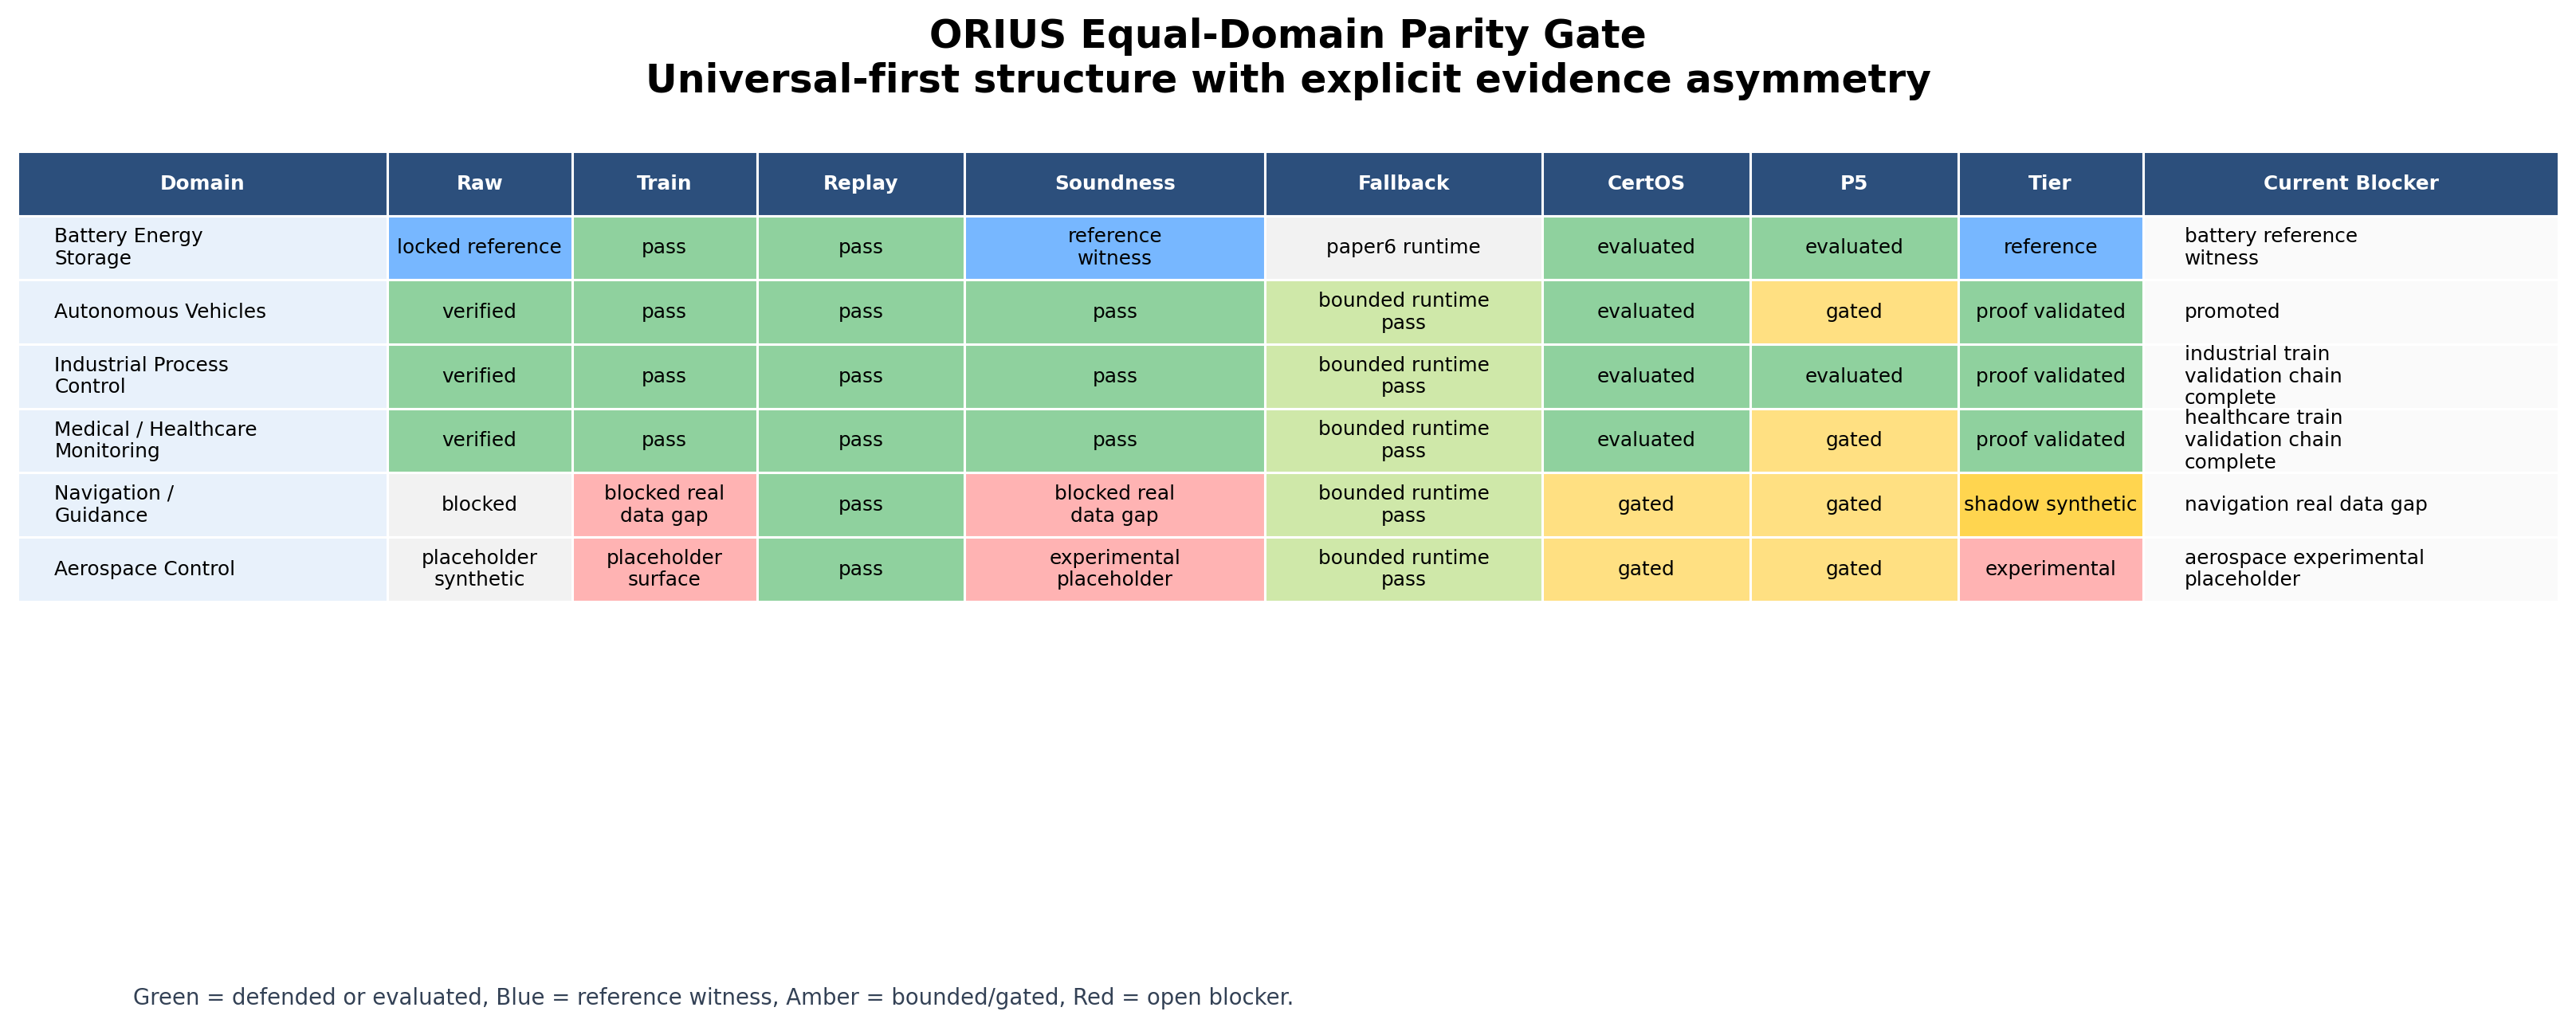
\includegraphics[width=0.92\textwidth]{fig_orius_equal_domain_parity_matrix}
\caption{Parity-gated view of the ORIUS program. The architecture is universal now, but
domain promotion remains governed by closure status rather than by rhetorical symmetry.}
\label{fig:prof-parity-visual}
\end{figure*}

The synthesis that follows from this status is narrower and stronger than a generic
transfer-learning claim.  ORIUS standardizes the runtime objects that matter for
safety under degraded observation:
reliability assessment, uncertainty widening, admissible-set tightening, repair or
fallback, certificate emission, and auditable lifecycle logging.  What varies across
domains is the safety geometry, the telemetry parser, and the domain-specific repair
policy.  What stays invariant is the safety-layer grammar.

That distinction is the key cross-domain result.  Battery remains the witness row, but
it does not monopolize the theory.  Industrial and healthcare are defended bounded
rows with real replay evidence.  Autonomous vehicles are defended under the current
bounded TTC contract.  Navigation and aerospace are still informative because they
show where the parity gate has not yet been earned.

The professor-facing takeaway is therefore precise: ORIUS already supports a
universal safety architecture, but the evidence ladder is still tiered.  The
architecture is universal in contract; the closure depth is not yet universal in
proof.  That is exactly the right level of honesty for an R1-grade monograph.

\subsection{Why ORIUS is more than a multi-domain wrapper}
Many systems can be described across multiple domains if the description remains
qualitative enough. ORIUS aims at a stronger standard. It keeps the same runtime
question, the same typed release objects, and the same benchmark semantics across all
rows. That is why the framework should be understood as universal in \emph{runtime
logic} rather than merely broad in \emph{application count}. The universal claim does
not come from listing six domains. It comes from showing that the same degraded-
observation semantics survive contact with six different action geometries.

\subsection{Autonomous vehicles}
The AV row treats degraded observation as a time-to-collision and entry-barrier hazard
under bounded vehicle semantics. Its runtime object is not the full autonomy stack. It
is the release decision under uncertain headway and environment state. The defended
bounded-row result matters because it shows the ORIUS contract moving into a
fast-reacting closed-loop domain without importing battery-specific actuation logic. The
row is bounded intentionally: the claim is about governed braking or maneuver legality,
not full autonomy closure.

\subsection{Industrial process control}
The industrial row treats degraded observation as envelope-preservation risk under
process telemetry loss or drift. The safety object is bounded operation inside process
constraints with explicit fallback semantics. This row demonstrates that ORIUS can
govern a plant whose action geometry and monitoring cadence look nothing like a storage
asset. Its universality contribution is that the repair operator can be phrased as
power-cap or envelope-preserving modification rather than storage dispatch logic.

\subsection{Healthcare monitoring}
The healthcare row is the clearest reminder that ORIUS is not only about actuation-
heavy control. Here the danger is intervention suppression or alert illegality under
degraded vital-sign observation. The defended bounded-row result shows that the same
runtime grammar still applies when the safety object is intervention legality rather
than dispatch power. It also marks a clean scientific boundary: the paper is not
claiming bedside autonomy certification, only monitored intervention legality under a
bounded runtime contract.

\subsection{Navigation}
The navigation row frames degraded observation as corridor or trajectory-feasibility
risk under degraded localization. The adapter and replay harness already exist, which
means the runtime contract is portable. What is missing is the defended real-data
closure row. That is why navigation remains shadow-synthetic in the present paper.

\subsection{Aerospace}
The aerospace row frames degraded observation as flight-envelope preservation under
degraded sensing and prognostic uncertainty. Its current role is boundary-setting: the
runtime objects and fallback semantics are already expressible, but the defended
multi-flight validation surface is not yet closed. Keeping aerospace visible but gated
is scientifically stronger than overstating parity.

\section{Explicit Evidence Boundary}
\label{sec:prof-evidence-boundary}

The manuscript does not overrun repository truth. The current repo supports a
universal runtime-safety architecture, but it does not support a flat claim
of equal empirical maturity across all six domains. The evidence boundary is
therefore part of the scientific contribution, not a defensive footnote.

\begin{table*}[t]
\centering
\caption{Allowed claims versus non-claims at the current evidence boundary.}
\label{tab:prof-evidence-boundary}
\small
\begin{tabularx}{\textwidth}{@{}p{0.24\textwidth}p{0.34\textwidth}p{0.34\textwidth}@{}}
\toprule
\textbf{Claim family} & \textbf{Supported by current repo truth} & \textbf{Not supported yet}\\
\midrule
Universal runtime grammar & One adapter contract, one benchmark schema, one CertOS lifecycle, and one degraded-observation hazard model across all rows. & A claim that all rows have identical proof depth or equal closure.\\
Battery witness depth & Deep theorem-to-code-to-artifact lineage with locked reference artifacts. & Treating battery as the conceptual center of the paper.\\
AV / industrial / healthcare & Defended bounded rows with locked replay and bounded runtime semantics. & Unqualified claims of unrestricted deployment readiness.\\
Navigation & Portability and protocol design evidence with a visible real-data gap. & Field-grade navigation validation or parity with the defended rows.\\
Aerospace & Experimental boundary evidence plus supplemental runtime diagnostics. & Proof-candidate or proof-validated aerospace closure.\\
\bottomrule
\end{tabularx}
\end{table*}

The tracked matrices make the boundary explicit. In
\texttt{reports/publication/orius\_equal\_domain\_parity\_matrix.csv}, battery is the
reference witness, autonomous vehicles, industrial process control, and healthcare
monitoring are defended bounded rows, navigation is shadow-synthetic, and aerospace is
experimental. The runtime-budget matrix and the universal validation summary say the
same thing in a different form: AV, industrial, and healthcare clear their bounded
contracts; navigation remains blocked by the missing real-data row; and aerospace
remains gated by the lack of a real multi-flight safety task with material post-repair
improvement.

The paper therefore uses the following claim discipline:
\begin{itemize}
  \item It may claim a universal safety layer for Physical AI under degraded observation.
  \item It may claim bounded validation for AV, industrial, and healthcare under their current contracts.
  \item It may claim portability and protocol design for navigation.
  \item It may claim experimental boundary evidence for aerospace.
\end{itemize}

It does not claim equal-domain universality, universal hardware closure, or field
deployment readiness for the navigation and aerospace rows.  Those would outrun the
present repository evidence and the locked validation outputs.

The practical implication is straightforward.  The manuscript can be ambitious about
architecture, but it must stay conservative about closure.  That is not a weakness in
the ORIUS program.  It is the reason the program remains defensible under serious
review.

\section{Conclusion}
\label{sec:prof-conclusion}

ORIUS argues that the right universal object for Physical AI safety is not a single
controller, a single benchmark, or a single proof family. It is a runtime safety layer
that mediates degraded observation before actuation. Once telemetry reliability becomes
part of the safety problem, the system must expose reliability, uncertainty inflation,
tightened action legality, repair, fallback, and certificate semantics as first-class
objects. That is the contribution of the Detect--Calibrate--Constrain--Shield--Certify
kernel.

The manuscript makes that contribution at three levels. First, it defines OASG as the
dominant hidden hazard: actions can remain legal on the observed state while becoming
unsafe on the true state. Second, it shows how a universal runtime contract can bind
adapter semantics, benchmark semantics, and CertOS governance under one typed layer.
Third, it demonstrates that the architecture is more than a diagram: the battery row
provides witness-depth theorem-to-code-to-artifact closure, and the defended bounded
rows show that the same runtime grammar travels beyond energy.

The scientific boundary is intentionally explicit. The paper does not claim equal-depth
closure beyond the defended three-domain lane. Battery is the witness row, and AV plus
Healthcare are bounded defended rows. Future additional domains remain outside the
current defended evidence package. That boundary does not weaken the architectural
thesis. It shows that ORIUS is disciplined enough to separate universality of contract
from the present evidence depth.

What changes at the field level is the object of research. ORIUS suggests that Physical
AI safety should be organized around reusable runtime layers that sit between nominal
intelligence and physical release. Such a layer can host conformal uncertainty, safety
filters, runtime assurance, and anomaly detection without collapsing into any one of
them. If future additional domains clear the same obligations, ORIUS supports a
broader empirical claim. Even before that point, it establishes a credible
safety-layer grammar for Physical AI under degraded observation.

In that sense, ORIUS is also a writing and evaluation proposal for the field. It argues
that future physical-AI systems should report not only predictive accuracy or planner
reward, but also true-state violation behavior, intervention frequency, fallback usage,
certificate validity, and release latency under degraded observation. That reporting
discipline matters because many failures in real systems are not failures of nominal
optimization; they are failures of release semantics once observation ceases to be
trustworthy. A framework like ORIUS makes those failures measurable and governable.


\newpage
\nocite{*}
\bibliographystyle{IEEEtran}
\bibliography{../bibliography/orius_monograph}

\end{document}
